\subsection{Status duration analysis}
  The duration distribution for each status are shown in fig.\ref{figure_duration_for_each_status}. Status duration represents the time length of a taxi staying in a certain status. The red line presents the duration time distribution for vacant status, and the green one is for status 1. A dot of the line means the proportion of the duration. A peak exists in each line, and it is obvious that the peak of the red line is earlier than that of the other line. And the value of duration for status 0 trends to be smaller. It accords to the realistic situation, because drivers tend to shorten the waiting time to raise their income.
\begin{figure}[!h]
\centering
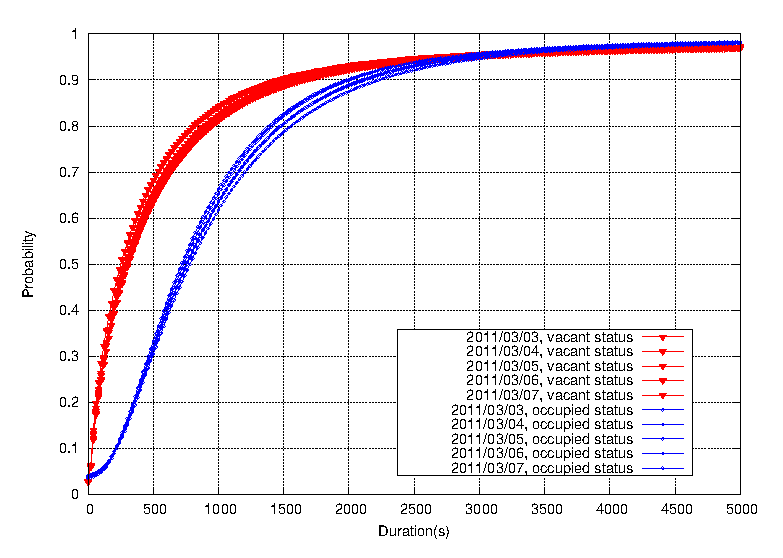
\includegraphics[width=0.3\textwidth]{figures_201103/assumption/durationdis.eps}\\
\caption{Status duration distribution.}\label{figure_duration_for_each_status}
\end{figure}

The statistical results are consistent with the \emph{assumption 1}, that is, the behaviors of taxis are similar within each status while it differs between the two statuses.
